\section{Resultados}
    \subsection{Metas propuestas con la tesis}
    Los resultados esperados para la investigación es que con base en la información recolectada en la fase de investigación de campo, se logre diseñar un modelo de datos e interfaces en computadora para la disposición del historial clínico del paciente que permita mejorar la calidad de la interacción paciente-médico y la interpretación de la semiología del paciente. Se espera que el modelo propuesto sea capaz de representar de manera efectiva la información del historial médico, garantizando la seguridad y trazabilidad de los datos.
    \subsection{Cronograma de Actividades}
    Para obtener los resultados que se pretenden alcanzar en el desarrollo del doctorado, se ha elaborado un cronograma de actividades que se detalla a continuación. Este cronograma está diseñado para guiar el progreso del proyecto y asegurar que se cumplan los plazos establecidos.
    \vspace{1em}

    \begin{figure} [H]
    \centering
    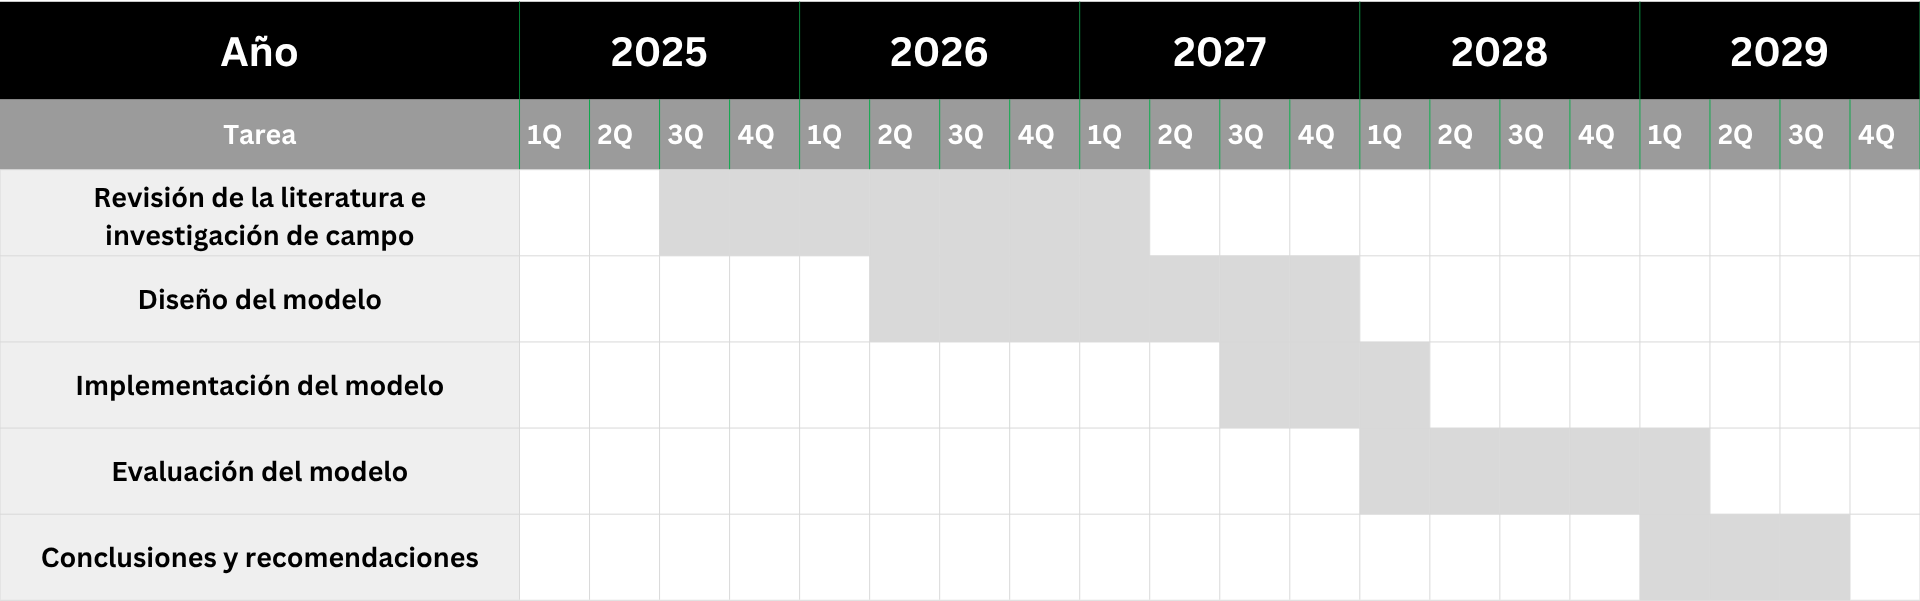
\includegraphics[width=0.9\textwidth]{images/gantt.png}
    \caption{Diagrama de Gantt del cronograma de actividades del Anteproyecto}    
    \end{figure}